\section{Applicazioni BIM su Desktop}
\label{sec:chapter_1_section_2}
Il panorama delle applicazioni Desktop, che implementa le funzionalità BIM e di modellazione è vasto.
Il software più noto e l’attuale leader di mercato BIM nella
progettazione architettonica è Autodesk Revit. Questo è il movito per il quale si è scelto questo framework parametro di confronto.

\subsection*{Autodesk Revit}
\label{sec:chapter_1_section_2_sub_1}
Autodesk \emph{Revit} è un programma CAD e BIM per sistemi operativi Windows, creato dalla Revit Technologies Inc. e comprato
nel 2002 dalla Autodesk per 133 milioni di dollari, che consente la progettazione con elementi di modellazione parametrica
e di disegno.
Revit negli ultimi sette anni ha subito profondi cambiamenti e miglioramenti. Prima di tutto, esso è stato modificato per poter
supportare in maniera nativa i formati DWG, DXF e DWF. Inoltre, è stato migliorato in termini di velocità ed accuratezza di
esecuzione dei rendering. A tal fine, nel 2008 il motore di rendering esistente, AccuRender, è stato sostituito con Mental Ray.
Tramite la parametrizzazione e la tecnologia 3D nativa è possibile impostare la concettualizzazione di architetture e forme
tridimensionali. Questo nuovo paradigma comporta una rivoluzione nella percezione progettuale, poiché questa si sostanzia in
termini non più cartesiani ma spaziali, con i vantaggi che questa può apportare alla progettazione~\cite{BIMrevolution}.
Revit, come programma BIM, (come si vede in Figura~\ref{fig:revit1}) è da intendersi come un approccio più vicino alla realtà
percepita dal uomo.
Uno dei punti di forza di Revit è quello di poter generare con estrema facilità viste prospettiche o assonometriche, che
richiederebbero notevoli sforzi nel disegno manuale; un esempio è la creazione di spaccati prospettici ombreggiati.
Altra caratteristica di estrema importanza è quella di costruire il modello utilizzando elementi costruttivi, mentre
in altri software analoghi la creazione delle forme è svincolata dalla funzione costruttiva e strutturale.
Elemento portante di Revit è lo sfruttamento della "quarta dimensione", cioè il tempo. Si possono infatti impostare le fasi
temporali: ad esempio, Stato di Fatto e Stato di Progetto. Ogni elemento del modello può essere creato in una fase e demolito
in un'altra, avendo poi la possibilità di creare viste di raffronto con le opportune evidenziazioni: "Gialli e Rossi".
I punti deboli del programma sono rappresentati, invece, dall'interfaccia talvolta poco intuitiva e dalla qualità dei rendering,
che, pur utilizzando il motore "radiosity", che fornisce un illuminazione globale del modello, non è paragonabile
a quella ottenibile con software di rendering dedicati.\\

\begin{figure}[htbp] %  figure placement: here, top, bottom, or page
   \centering
   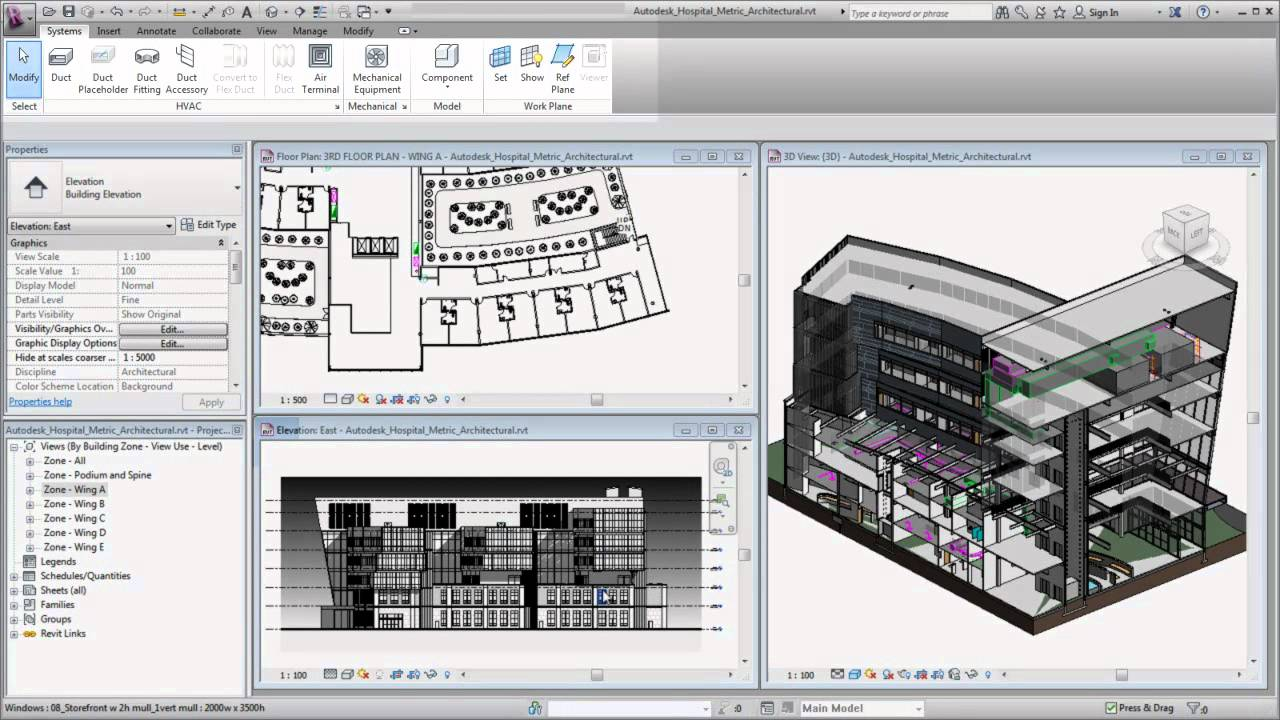
\includegraphics[width=1\linewidth]{images/maxresdefault}
   \caption{Schermata Autodesk Revit}
   \label{fig:revit1}
   \end{figure}
   \newpage
